\documentclass{article}
\usepackage{hyperref}
\usepackage{graphicx}
\usepackage{float}
\usepackage{caption}
\usepackage{graphicx}
\usepackage[utf8]{inputenc}
\usepackage[T1]{fontenc}

\title{Predykcja wypadków samochodowych w Polsce\\w latach 2018-2023\\na podstawie danych pogodowych}
\author{Jakub Śliwka 272549\\Informatyka Stosowana\\Wydział Informatyki i Telekomunikacji}
\date{10 Czerwiec 2022}

\usepackage[a4paper, left=2cm, right=2cm, top=3cm, bottom=3cm]{geometry}

\begin{document}

\maketitle

\section{Wstęp}

Polska jest jednym z czołowych krajów w Europie pod względem liczby śmiertelnych wypadków samochodowych w przeliczeniu na milion mieszkańców.
Pod tym względem tylko Rumunia, Bułgaria, Litwa i Chorwacja mają gorsze statystyki.
Wypadki drogowe są jedną z głównych przyczyn zgonów w Polsce, dlatego celem projektu jest analiza wypadków samochodowych oraz stowrzenie modelu zdolnego przewidzieć liczbę wypadków na podstawie specjlanych warunków. 
W kolejnych rozdziałach przybliżę temat wypadków samochodowych, przeanalizuję czynniki zewnętrzne takie pogoda, weekendy czy święta



\section{Dane użyte w programie}

Dane pogodowe używane w projekcie zostały pobrane ze strony
\url{https://danepubliczne.imgw.pl} w formie \textit{zip}. Program automatycznie rozpakowywuje pliki oraz łączy je w jeden plik \textit{csv}.

Dane o wypadkach zostały \textit{zescrapowane} ze strony \url{https://policja.pl/}. Program wyszukuje strony z odpowiednimi datami i dzięki bibliotece \textit{BeautifulSoup} wyszukuje tabelkę z odpowiednimi danymi, po czym łączy i zwraca \textit{DataFrame}. 

Dane o świętach w Polsce zostały \textit{zescrapowane} ze strony \url{https://www.timeanddate.com/holidays/poland/}. Tutaj również została użyta biblioteka w Pythonie \textit{BeautifulSoup} do wyszukania odpowiedniej tabeli zawierającej dane o świętach w Polsce.

Dane o weekendach zostały wyszukane za pomoca biblioteki \textit{Pandas} przy pomocy \textit{DataFrame}'ów

\section{Analiza danych}
\subsection{Wypadki drogowe}
\subsubsection{Liczba wypadków}
Analizę danych warto rozpocząć od samych wypadków drogowych.

\begin{center}
    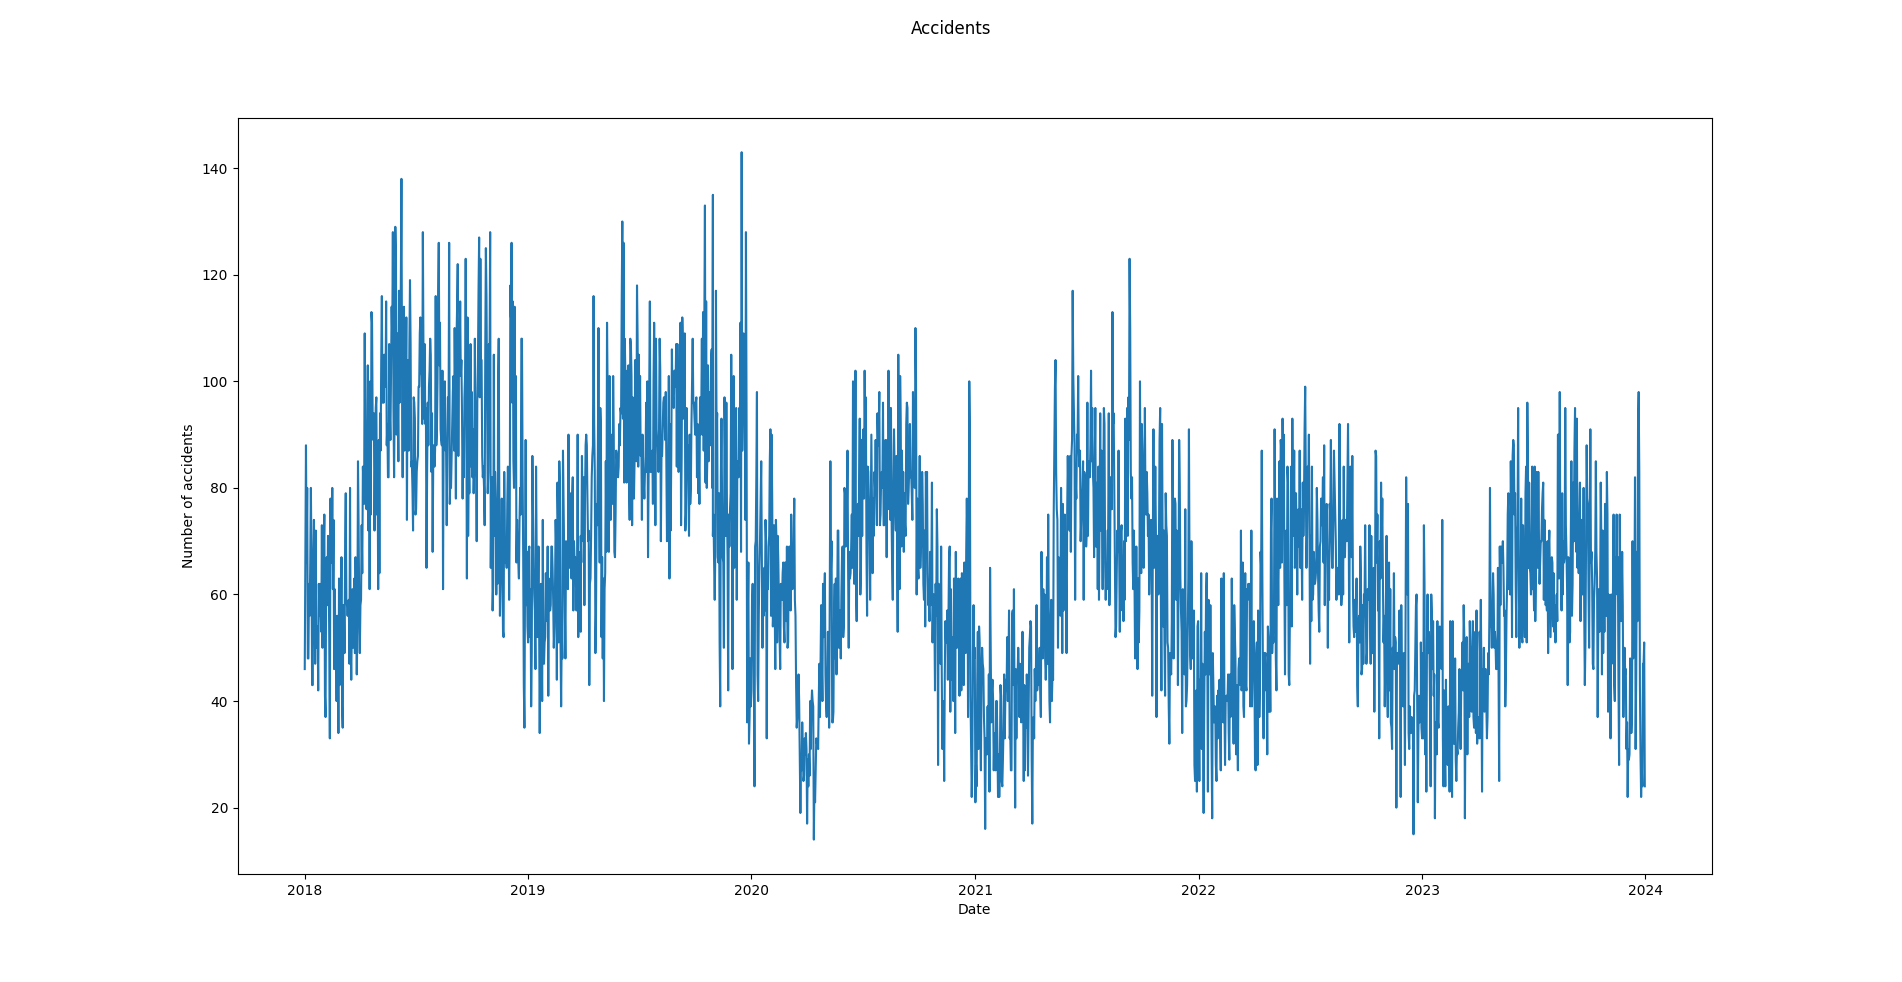
\includegraphics[width=\textwidth]{visualization/accidents.png}
    \captionsetup{hypcap=false}
    \captionof{figure}{Ilość wypadków w latach 2018-2023}
    \label{fig:accidents}
\end{center}

Widząc wykres \ref{fig:accidents} od razu można zuważyć tendencje spadkową. Ponadto wykres przypomina sinusoidę. Bez żadnych dodatkowych informacji, można dostrzec, że w okresie letnim wypadki zdarzały sie dużo częściej, niż w okresie zimowym. Sugeruje to, że w trudniejszych warunkach kierowcy są bardziej ostrożni.

\begin{center}
    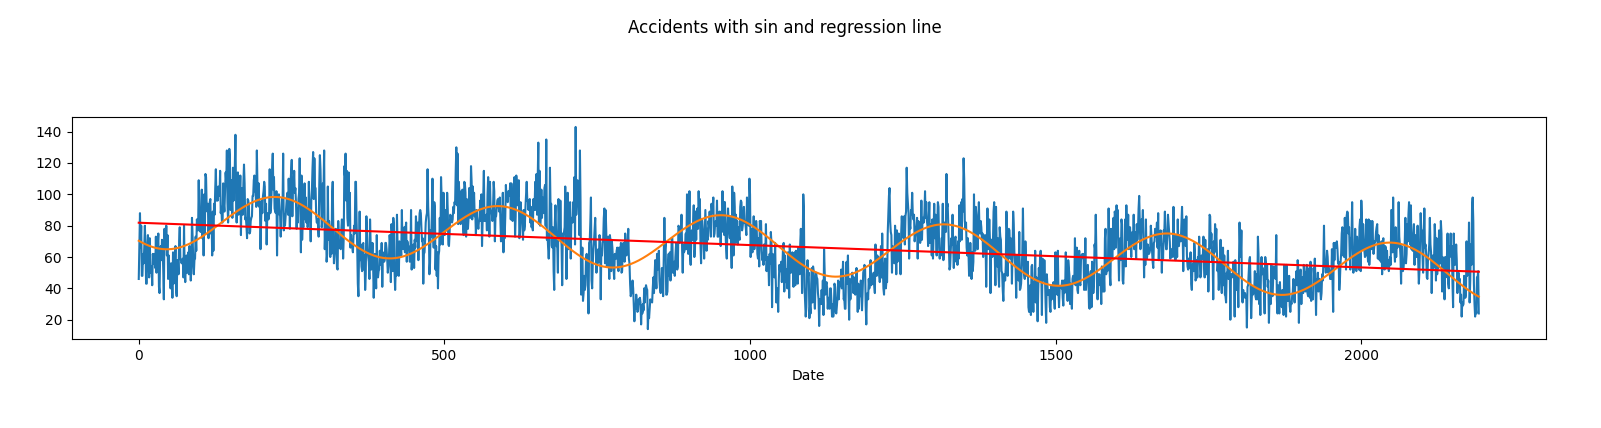
\includegraphics[width=\textwidth]{visualization/accidents_sin.png}
    \captionsetup{hypcap=false}
    \captionof{figure}{Wykres liczby wypadków drogowych z linią regresji oraz funkcją sinusoidalną}
    \label{fig:accidents_sin}
\end{center}
Na wykresie \ref{fig:accidents_sin} 0 oznacza 01.01.2018, natomiast końcowa wartość to 31.12.2023

Na wykresie \ref{fig:accidents_sin} została dodana linia regresji oraz sinusoida dopasowana do wykresu wypadków. Jak widać wykres ma tendencję spadkową. Funkcja sinusoidalna w przybliżeniu prezentuje sie wzorem:

\begin{equation} \label{eq:sin_equation}
    y = -0.016x + 84 + 12\sin(0.017x - 231) 
\end{equation}

Warto jednak zbadać dokładniej wykres \ref{fig:accidents}. Poniżej zostały zamieszczone wykresy dzielące okresy na lata oraz miesiące

\begin{center}
    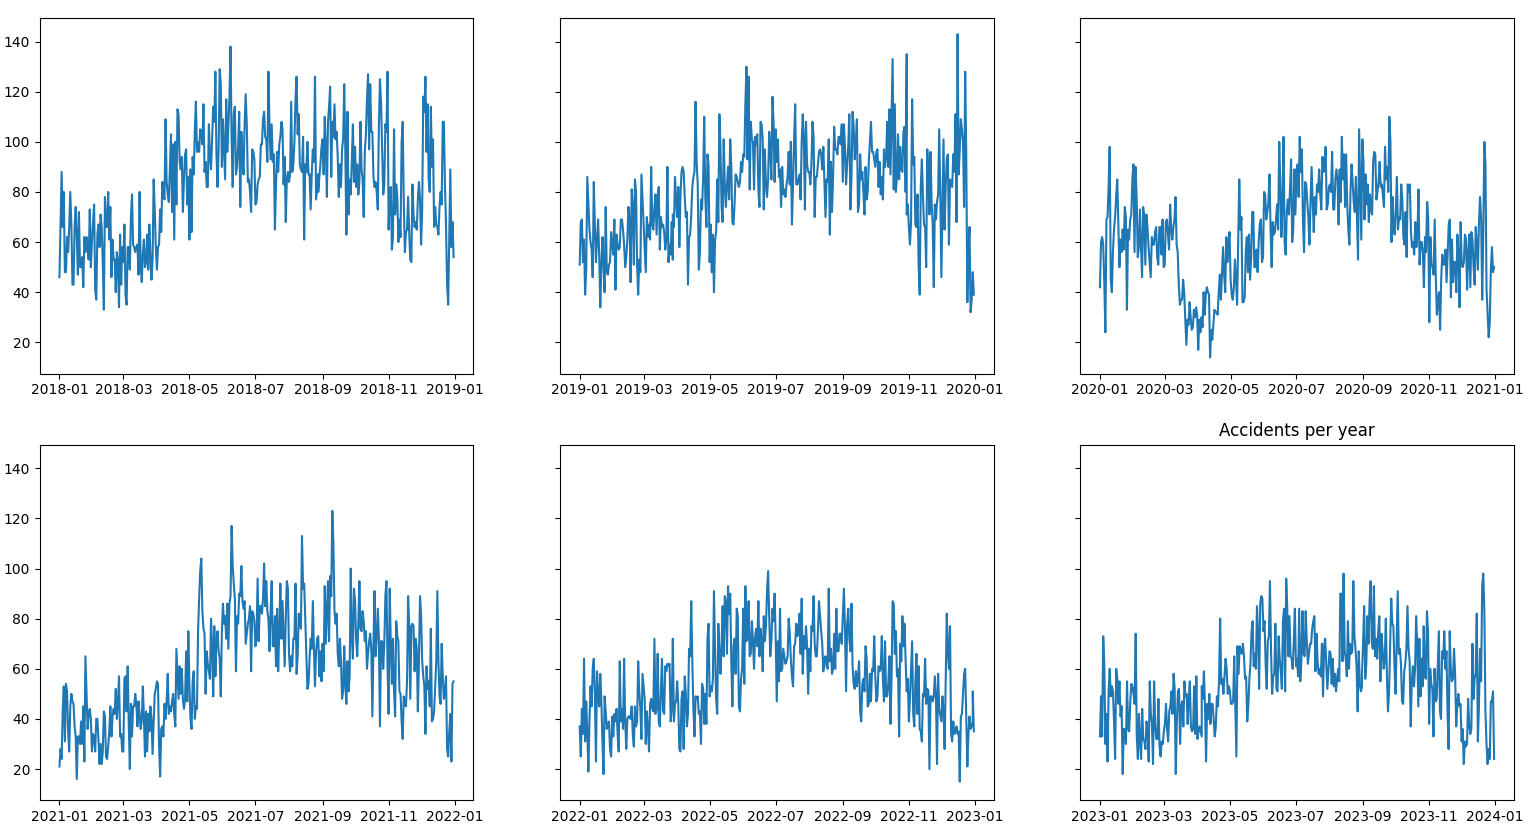
\includegraphics[scale=0.3]{visualization/accidents_per_year.png}
    \captionsetup{hypcap=false}
    \captionof{figure}{Wykres wypadków drogowych podzielony na lata od 2018-2023}
    \label{fig:accidents_year}
\end{center}

\begin{center}
    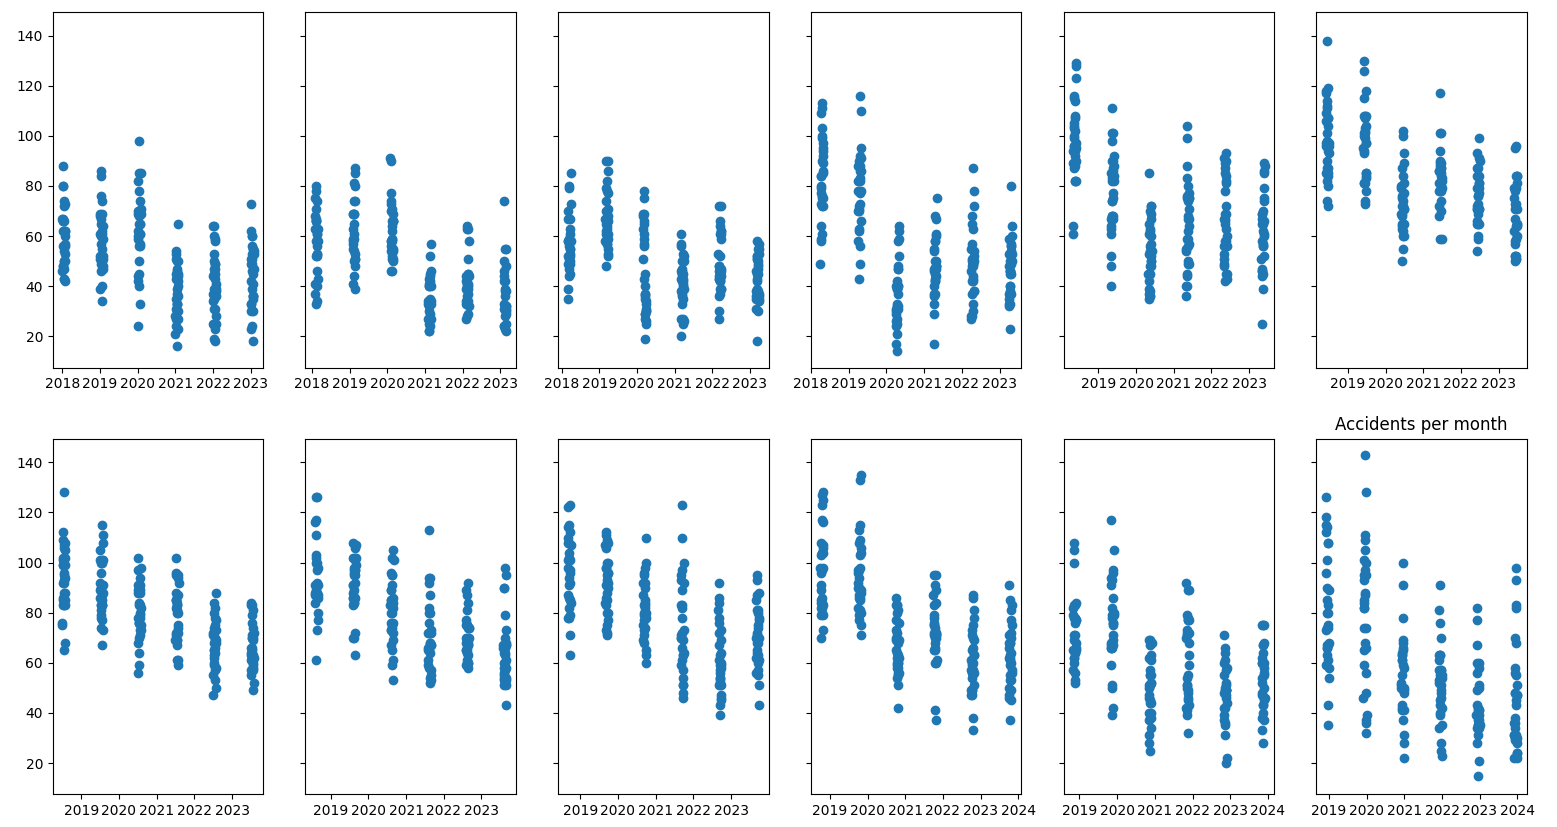
\includegraphics[scale=0.3]{visualization/accidents_per_month.png}
    \captionsetup{hypcap=false}
    \captionof{figure}{Wykres wypadków drogowych w miesiącach}
    \label{fig:accidents_month}
\end{center}

Wykresy \ref{fig:accidents_year}, \ref{fig:accidents_month} prezentuja jak w następnych latach zmieniały się wypadki w Polsce. W 2020 roku na przełomie marca oraz kwietnia można dostrzec nagły spadek wypadków drogowych. Było to spowodowane lockdown'em wprowadzonym wówczas z powodu pandemii. Załamanie "Covidowe" widoczne jest również na wykresie \ref{fig:accidents_month}. 
W latach 2022-2023 gdy obostrzenia "Covidowe" były powoli łagodzone, ilość wypadków nie zaczęła ulegać aż takiemu wzrostowi. Na ten fakt mógł mieć wpływ ingerencji rządu oraz zaostrzenia przepisów drogowych. Zmiany taryfikatorów drogowych mogły spowodować, zwiększenie ostrożności kierowców w obawie przed wysokimi mandatami.

Co równie ważne dobrze widoczne różnice o których mowa była wcześniej, czyli różnice w porach roku lato/zima

\begin{center}
    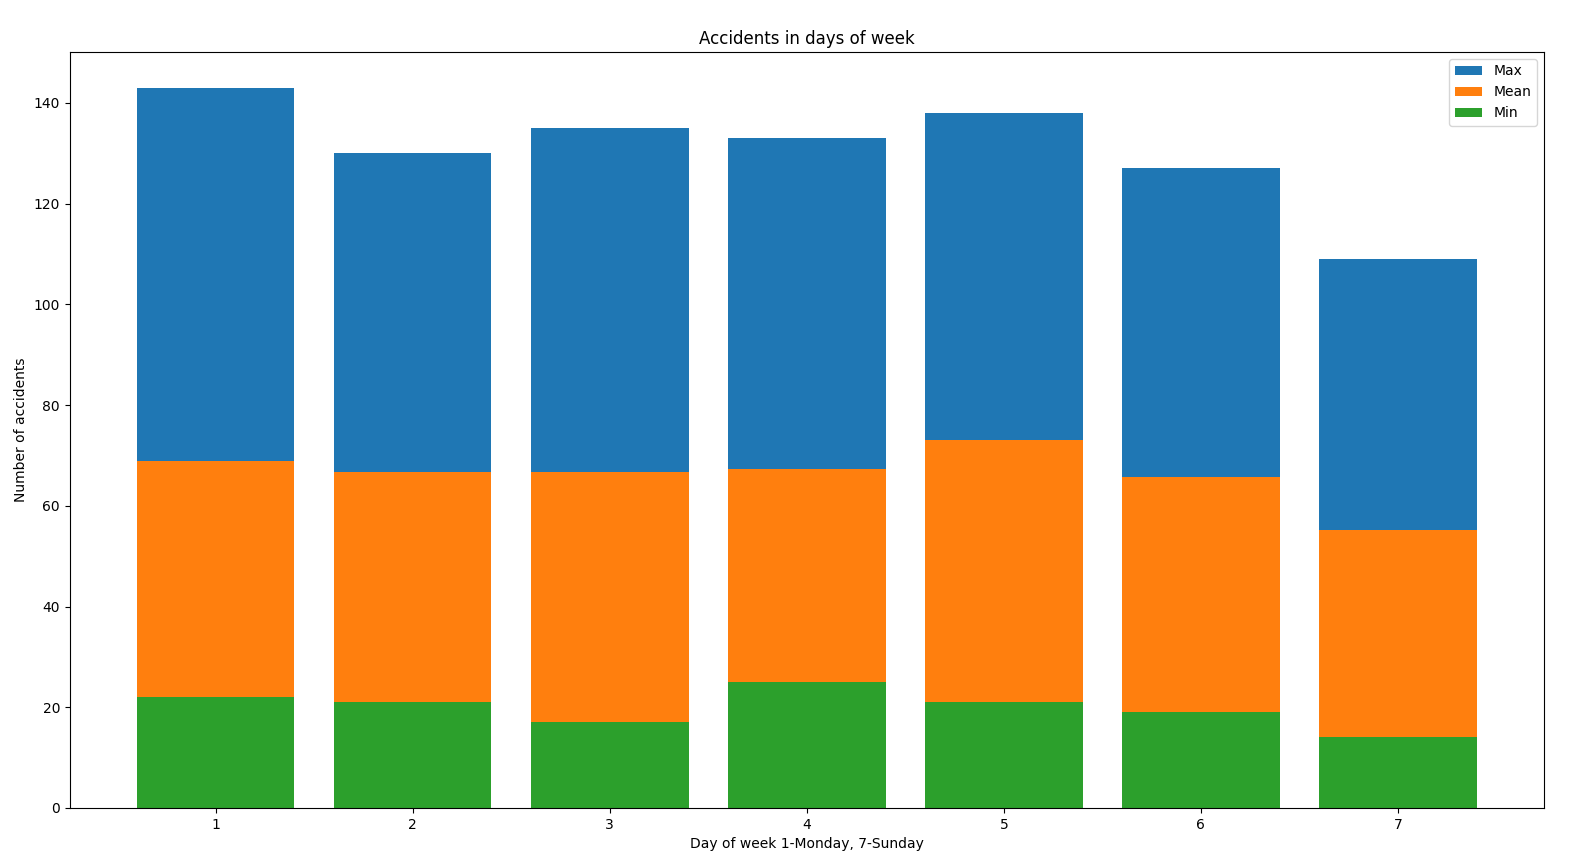
\includegraphics[scale=0.3]{visualization/accidents_days_of_week.png}
    \captionsetup{hypcap=false}
    \captionof{figure}{Wykres wypadków drogowych w dniach tygodnia}
    \label{fig:accidents_weeks}
\end{center}

\begin{center}
    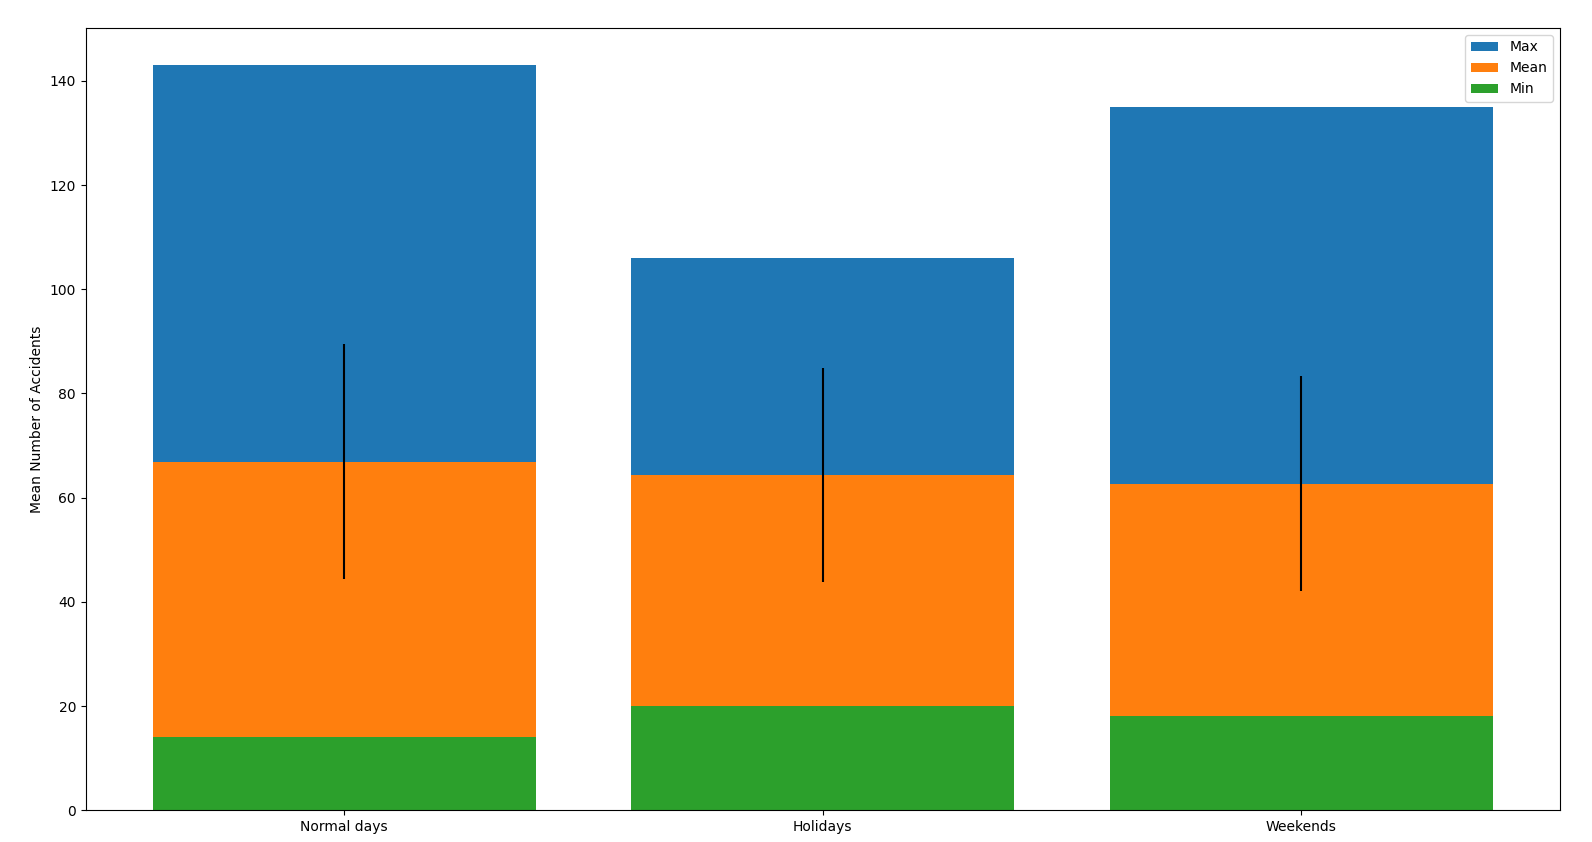
\includegraphics[scale=0.3]{visualization/normal_vs_holidays_vs_weekends.png}
    \captionsetup{hypcap=false}
    \captionof{figure}{Wypadki drogowe w poszczególnych rodzajach dni}
    \label{fig:accidents_types}
\end{center}

Z wykresu \ref{fig:accidents_weeks} widać, że średnio najwięcej wypadków wypadało w piątek. Może to wynikać z początku weekendu w czasie którym wiele osób planuje wyjazdy. Minimalne załamanie widać w Niedzielę. Może to być spowodowane kilkoma czynnikami, m.in. tym, że niedziela jest uważana za ważny dzień z powodu chrześcjiańskiego charakteru Polaków lub "odpoczynkiem" przed nadchodzącym tygodniem pracy.
Aż tak dużego znaczenia nie ma natomiast rodzaj dni. Nie ma znaczej różnicy między dnami powszednimi, świętami a weekedami. 

\subsubsection{Liczba poszkodowanych oraz śmierci}

Warto jest zająć się kwestią ilości poszkodowanych oraz śmierci w wypadkach samochodowych. Obie te kwestwie są mocno powiązane z ilością wypadków omawianych w poprzedniej sekcji. 

\begin{center}
    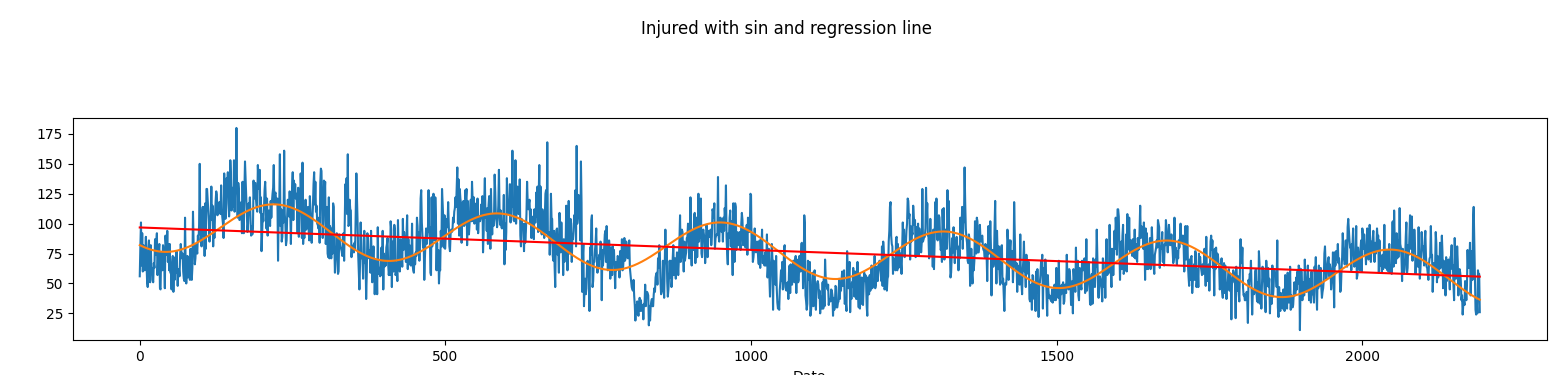
\includegraphics[scale=0.3]{visualization/injured_sin.png}
    \captionsetup{hypcap=false}
    \captionof{figure}{Wykres poszkodowanych w wypadkach drogowych}
    \label{fig:injured_death}
\end{center}

Wykres \ref{fig:injured_death} wygląda podobnie do wykresu \ref{fig:accidents}. Zauważalny jest również "Covidowe" załamanie. Wzór który można dopasować do wykresu jest podobny to poprzedniego.

\begin{equation} \label{eq:sin_equation2}
    y = -0.020x + 100 + 22\sin(0.017x - 235) 
\end{equation}


 \begin{center}
    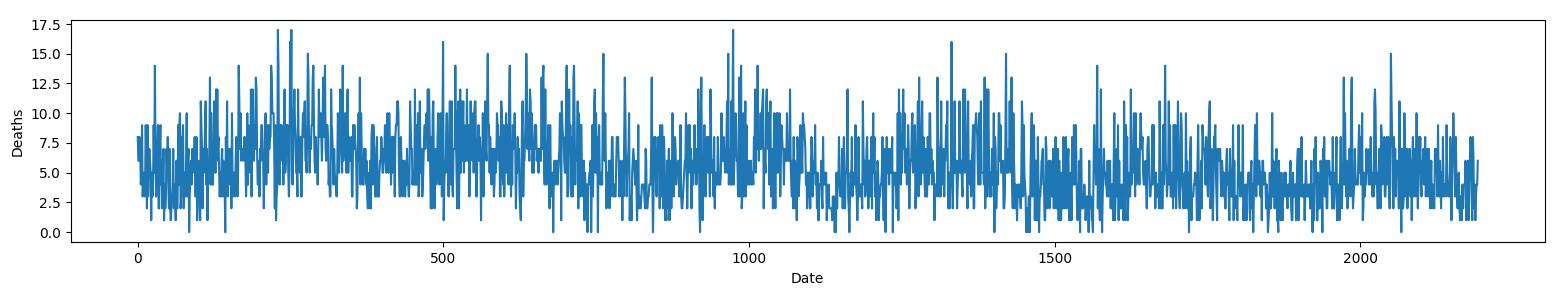
\includegraphics[scale=0.4]{visualization/deaths.png}
    \captionsetup{hypcap=false}
    \captionof{figure}{Wykres śmierci w wypadkach drogowych}
    \label{fig:deaths}
\end{center}

Wykres śmierci \ref{fig:deaths} rówież zależny jest od ilości wypadków. Jednak wspólnym czynnikiem który wpływa pośrednio lub bezpośrednio na wypadki, poszkodowanych i śmierci jest pora roku. Co za tym idzie pogoda. Warto zatem przyjżeć sie bliżej pogodzie w latach 2018-2023, być może to właśnie ona miała większy lub mniejszy wpływ na wypadki drogowe. 

\subsection{Pogoda}
\subsubsection{Temperatura powietrza}
Na poprzednich wykresach można było zauważyć korelację pomiędzy porami roku, 
a wypadkami samochodowymi. Dlatego warto najpierw przyjrzeć się temperaturze.

 \begin{center}
    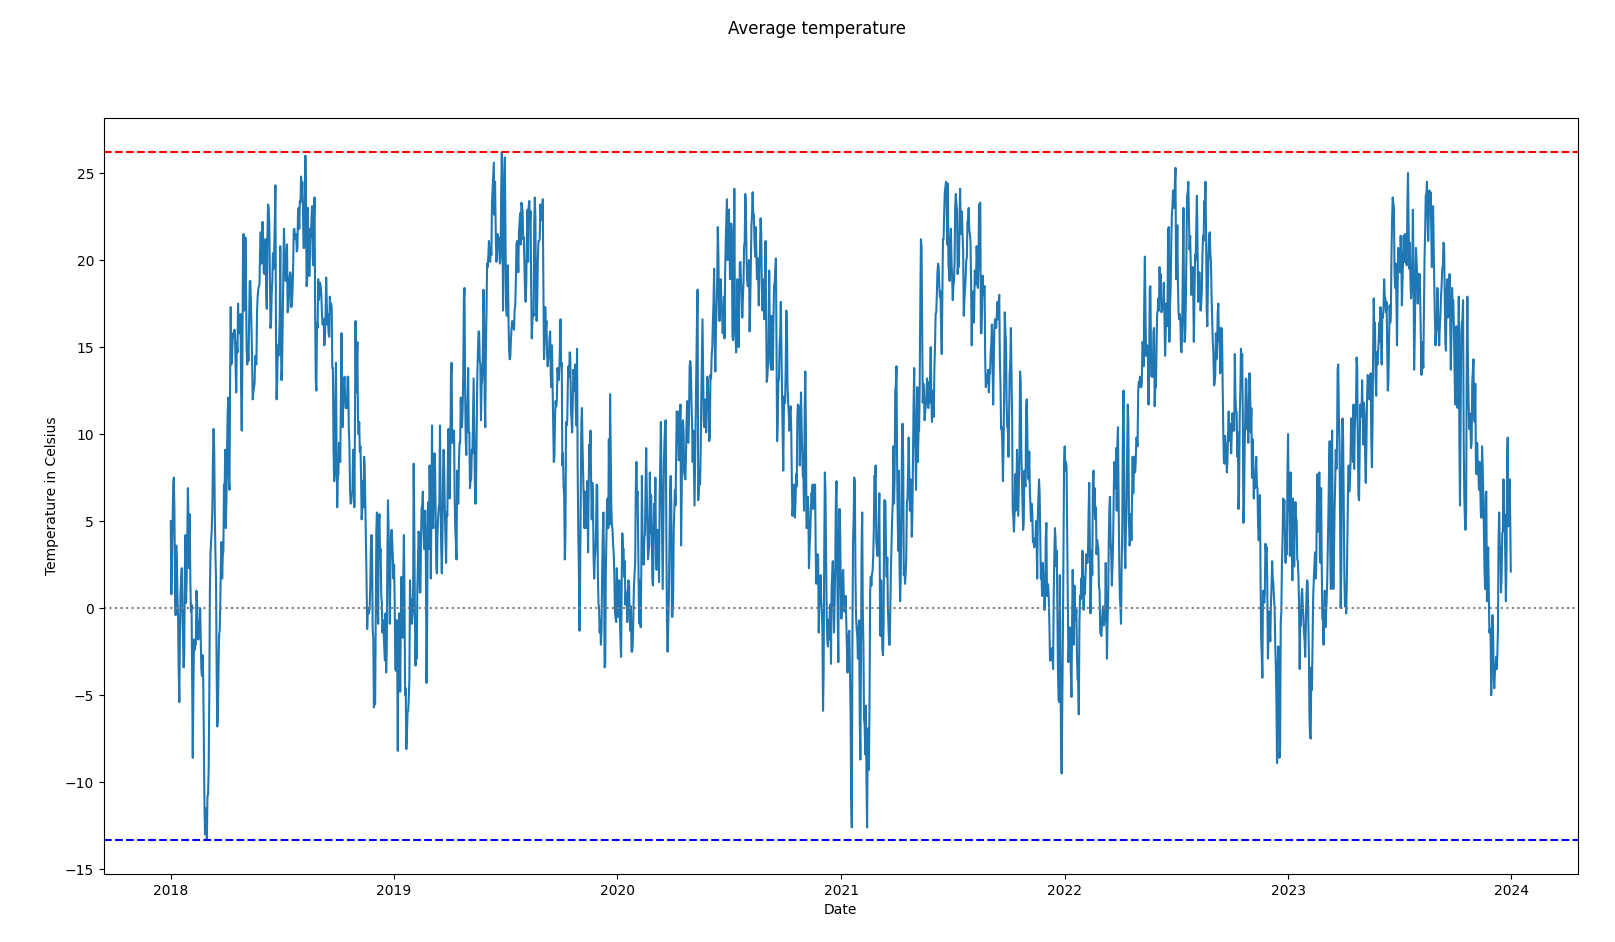
\includegraphics[scale=0.25]{visualization/avg_temp.png}
    \captionsetup{hypcap=false}
    \captionof{figure}{Temeratura w Polsce w latach 2018-2023}
    \label{fig:avg_temp}
\end{center}

Widząc wykres średniej temperatury dobowej w Polsce można zauważyć korelację między temperaturą dobową, a ilością wypadków w Polsce \ref{fig:accidents}. Przyglądając się obu wykresom można wysnuć wniosek, że pora roku a właściwie temperatura ma wpływ na ilość wypadków. 

 \begin{center}
    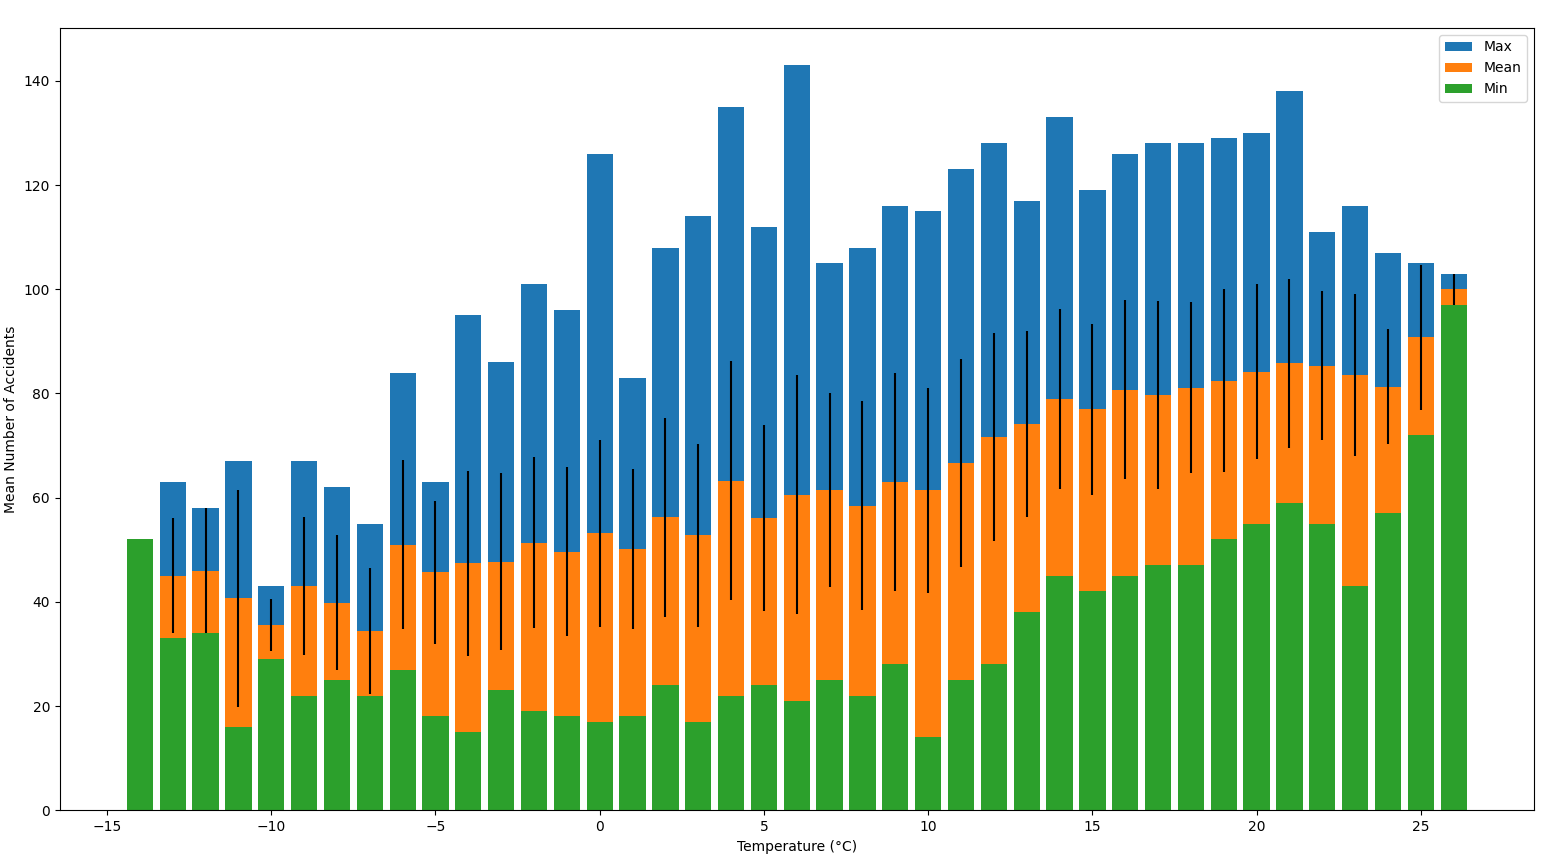
\includegraphics[scale=0.3]{visualization/temp_vs_accidents.png}
    \captionsetup{hypcap=false}
    \captionof{figure}{Temperatura oraz ilość średnia liczba wypadków}
    \label{fig:temp_vs_accidents}
\end{center}

 \begin{center}
    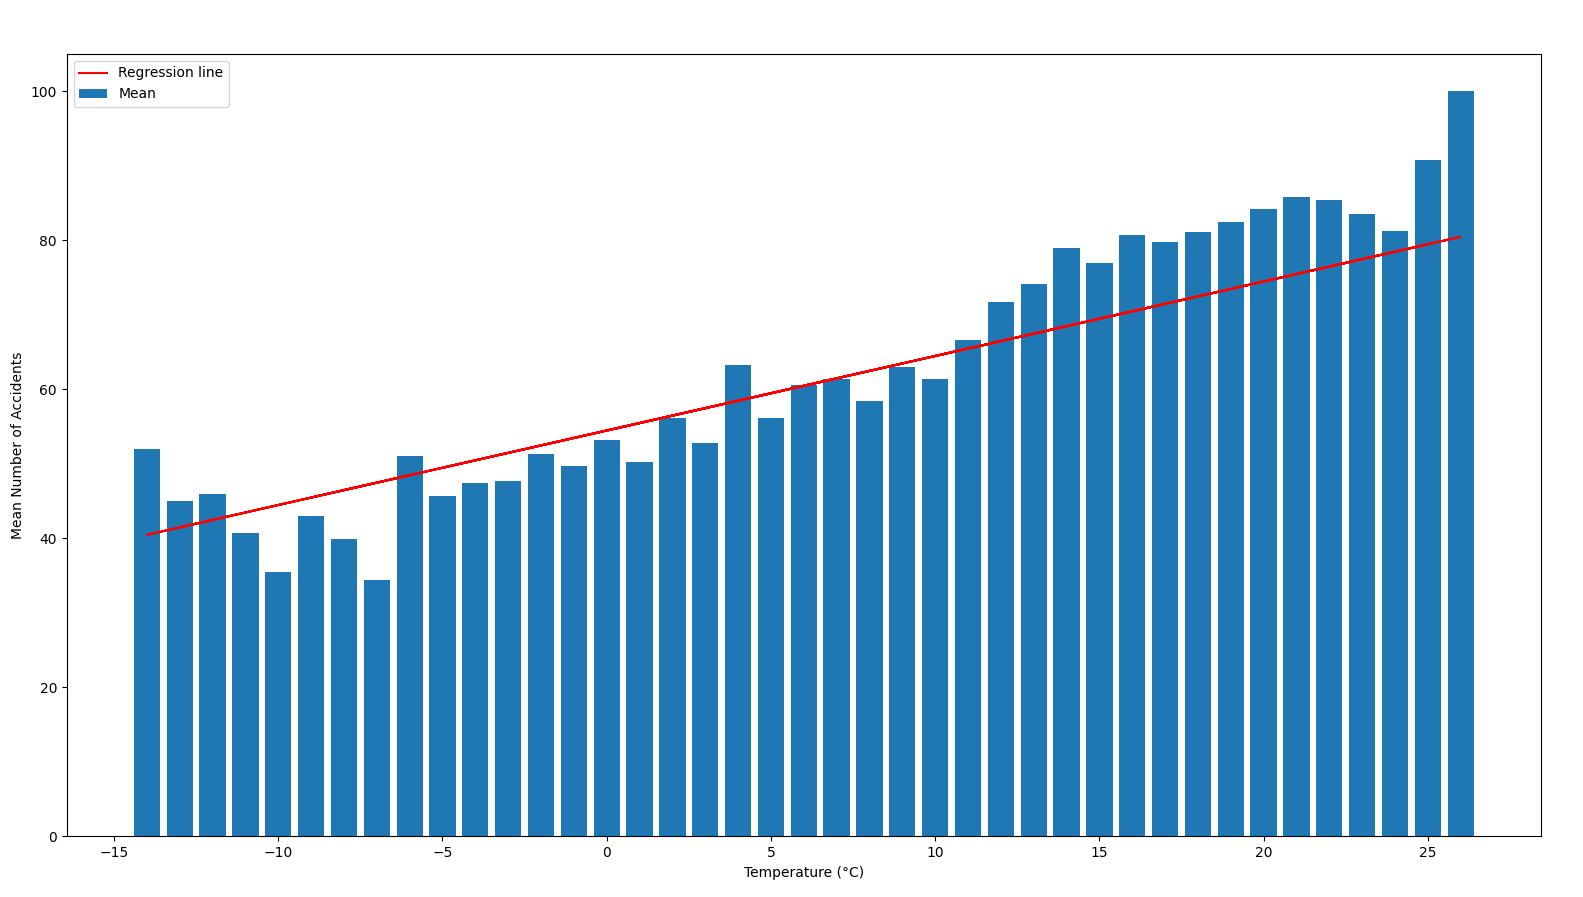
\includegraphics[scale=0.3]{visualization/temp_vs_accidents_regress.png}
    \captionsetup{hypcap=false}
    \captionof{figure}{Temperatura, ilość średnia liczba wypadków z linią regresji}
    \label{fig:temp_vs_accidents_regress}
\end{center}


Potwierdzenie tego wniosku można znaleźć w wielu źródłach np. \url{https://www.auto-swiat.pl/porady/kiedy-jest-najwiecej-wypadkow-na-drogach-odpowiedz-cie-zaskoczy/2gvz064}. Podczas trudniejszych warunków pogodowych, droga wymaga od kierowców ciągłego skupienia oraz koncentracji. Natomiast dobra pogoda usypia czujność kierowcóœ. Gdy widoczność jest dobra, nie pada deszcz, a ruch jest jednostajny, koncentracja kierowców maleje z czasem.

\subsubsection{Opady atmosferyczne}

Warto przypatrzeć sie również opadom atmosferycznym. Co statystyki mówią o wypadkach podczas deszczu? 

 \begin{center}
    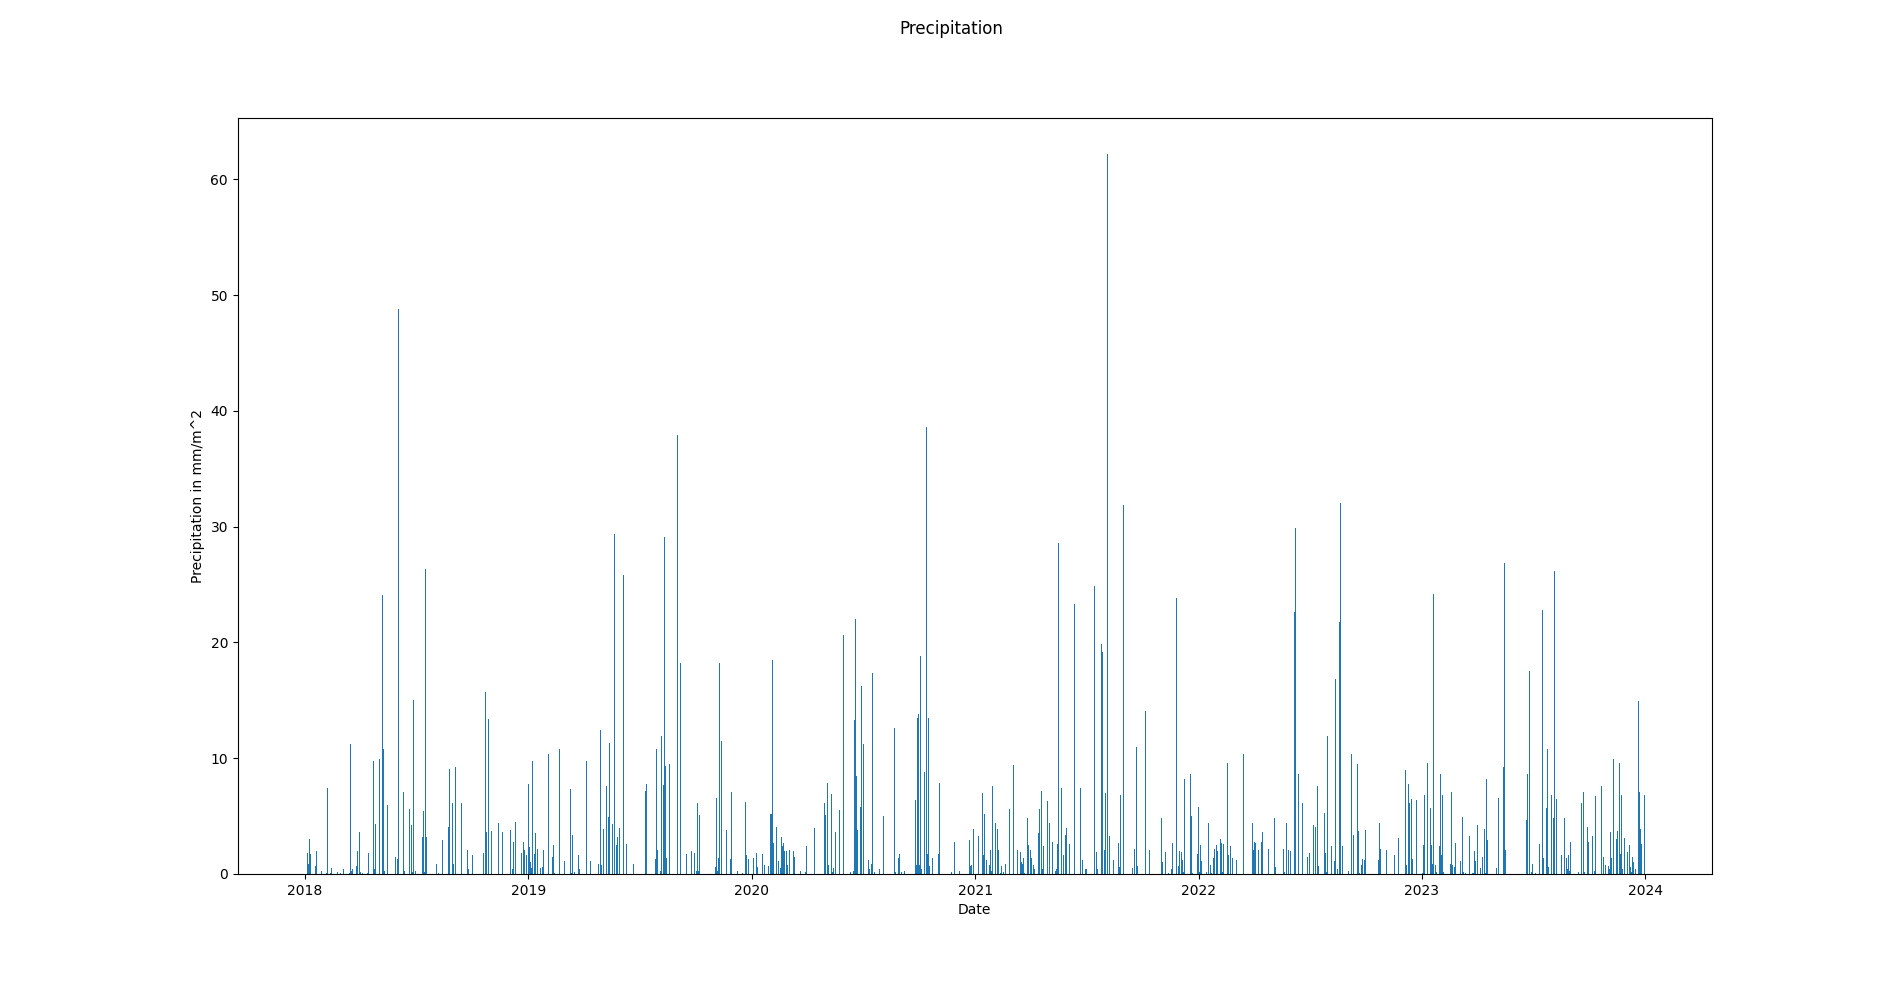
\includegraphics[scale=0.3]{visualization/precips.png}
    \captionsetup{hypcap=false}
    \captionof{figure}{Opady atmosferyczne w latach 2018-2023}
    \label{fig:precips}
\end{center}

 \begin{center}
    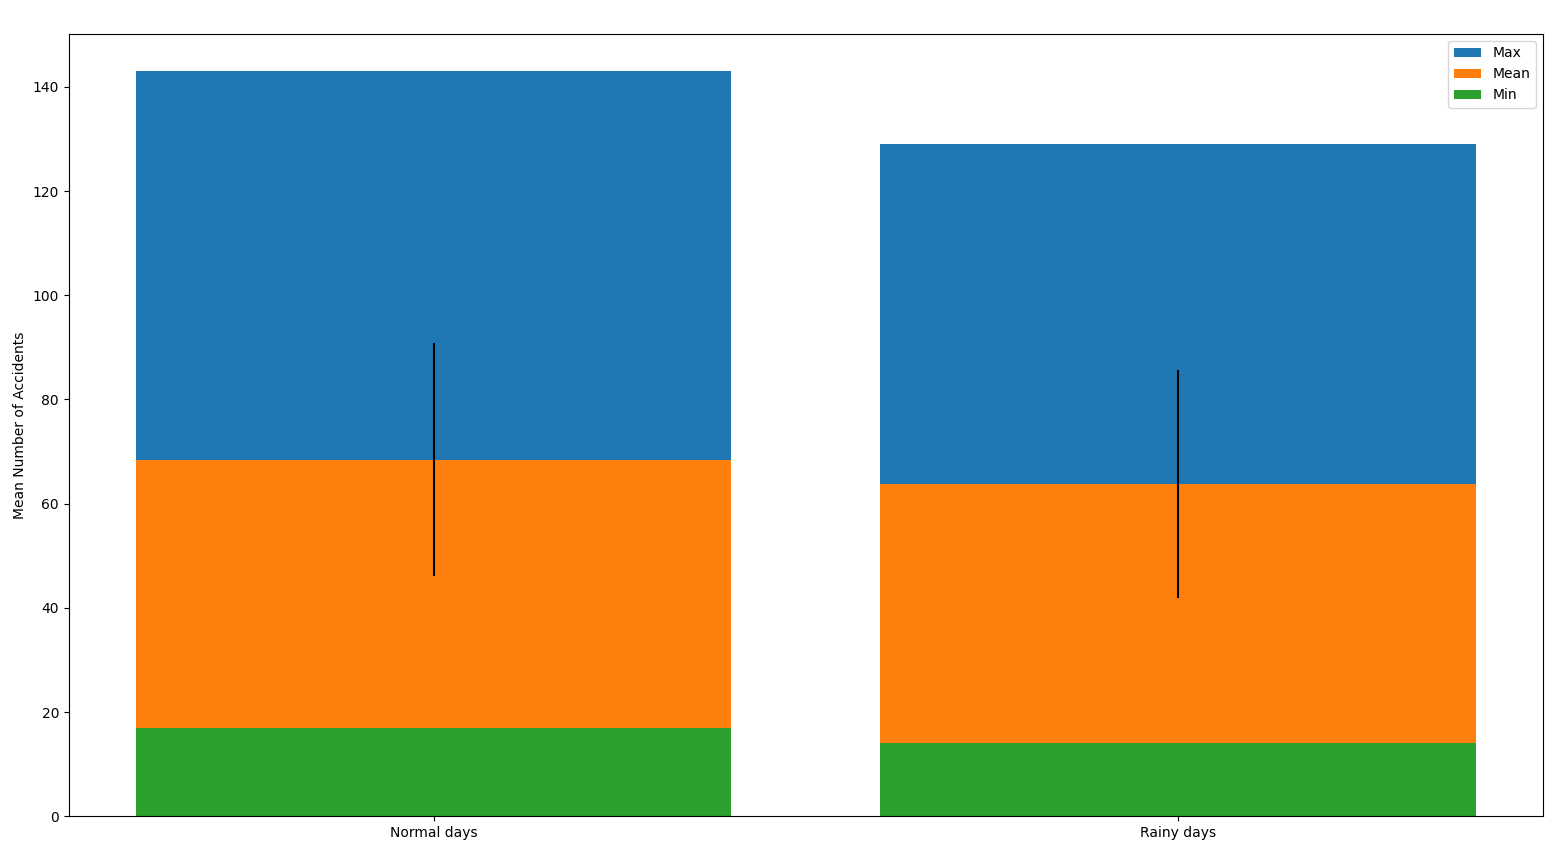
\includegraphics[scale=0.3]{visualization/normal_vs_rainy.png}
    \captionsetup{hypcap=false}
    \captionof{figure}{Wypadki podczas pogody oraz opadów}
    \label{fig:normal_vs_rainy}
\end{center}

Wykres \ref{fig:precips} prezentuje opady, na którym trudno doszukiwać się jakiejkolwiek korelacji.

Dużo ciekawszy jest natomiast wykres \ref{fig:normal_vs_rainy} na którym widać minimalną różnicę między średnią ilością wypadków w pogodne dni, a deszczowe.
Wykresy \ref{fig:normal_vs_rainy} oraz \ref{fig:temp_vs_accidents_regress} potwierdzają wniosek wysnuty w poprzednim rozdziale, że pogoda ma wpływ na ilość wypadków.

Czy rodzaj opadów wpływa na ilość wypadków? Takie pytanie pytanie może nasunąć się widząc wykres \ref{fig:normal_vs_rainy}. Warto zatem porównać te sobą deszcz oraz śnieg.

 \begin{center}
    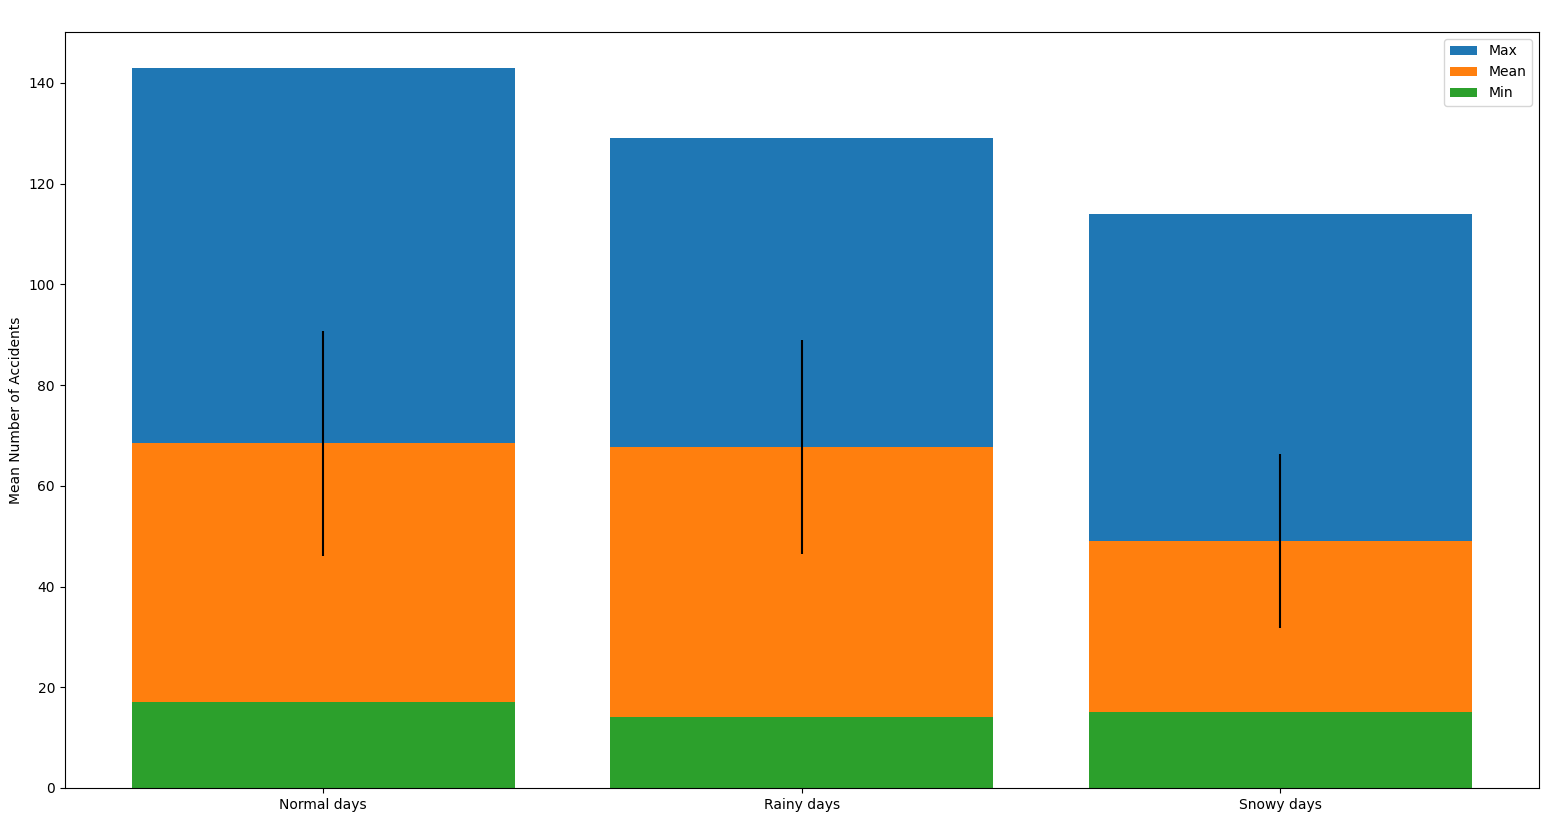
\includegraphics[scale=0.3]{visualization/rain_vs_snow.png}
    \captionsetup{hypcap=false}
    \captionof{figure}{Wypadki podczas pogody, deszczu, śniegu}
    \label{fig:normal_vs_rainy}
\end{center}
Jak widać opady śnegu mocno odbiegają od opadów deszczu. Średnia ilość wypadków jest prawie taka sama jak w dni pogodne. 

Na podstawie danych pogodowych można dojść do wniosku, że ładna pogoda sprzyja wypadkom. Natomiast podczas pory zimowej gdy droga wymaga ciągłego skupienia ilość wypadków jest znacznie mniejsza.

Jak zostało powiedziane, wiele czynników wpływa na wypadki samochodowe. Jednak czy za pomocą danych jakimi są zmienna pogoda, święta oraz weekendy, da się przewidzieć ilość wypadków, rannych oraz śmierci w Polsce?
To zagadnienie zostanie omówione w kolejnym rozdziale.

\section{Predykcja wypadków w Polsce}

Moim celem jest przewidzenie dokładnej ilości wypadków przy odpowiednich zadanych warunkach. Dlatego wybór padł na \textit{Regressor}'y

\subsection{Support Vector Regression}
Support Vector Regression (SVR) jest rodzajem Support Vector Machine (SVM). 

Ponieważ SVR jest algorytmem opartym na odległości, skalowanie jest ważnym etapem przetwarzania wstępnego, który może poprawić dokładność i stabilność modelu.
Dane które przyjmuje SVR powinny być wstępnie przetworzone, przeskalowane, ponieważ model bazuje na odległości. Do skalowania użyty zostały StandardScaler. Moduł ten  skaluje dane tak, aby ich średnia wynosiła 0, a odchylenie standardowe wynosiło 1.


SVR oryginalnie został stworzony jako single-output, chcąc przewidzieć ilość wypadów, rannych i śmierci można użyć \textit{MultiOutputRegressor}, który działa jak wrapper na SVR i rozszerza do multi-output. 

 \begin{center}
    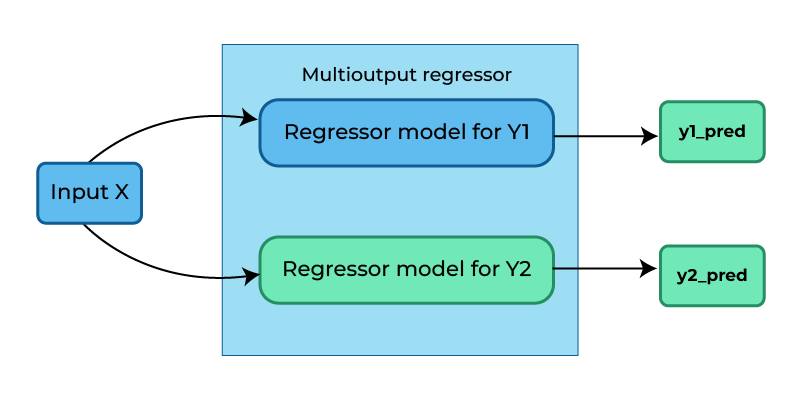
\includegraphics[scale=0.4]{images/multioutput-regression-02.png}
    \captionsetup{hypcap=false}
    \captionof{figure}{\href{https://www.geeksforgeeks.org/multioutput-regression-in-machine-learning/}{www.geeksforgeeks.org}}
    \label{fig:multioutput}
\end{center}

Wyszukując najlepsze parametry zdałem się na GridSearchCV. Testując parametry na modelach zwrócił wartości najlepsze parametry: kernel=rbf, gamma=10, C=4.
Scoring jaki został użyty w GridSearchCV to \textit{mean absolute error}


\subsection{Random Forest Regression}
Random Forest to metoda uczenia się zespołowego, która łączy predykcje z wielu drzew decyzyjnych w celu uzyskania dokładniejszych i stabilnych wyników. Random Forest używa się zarówno do Regresji jak i Klasyfikacji.

Random Forest składa sie z wielu Drzew Decyzyjnych. Każde drzewo ma tak zwane bootstrap samples. Bootstrap samples to podzbiór oryginalnego zbioru. Podzbiór ten to losowo wybierane dane.
Ważne jest żeby podzbiór ten finalnie zawierał rówież powtórzenia. Oczekuje się ~63,2\% unikalnych danych. 

Dla klażdego subsetu wybiera sie również podzbiór niepowtarzalnych cech. Każde drzewo jest trenowane. Wynik w przypadku regresji jest średnią, natomiast w przypadku klasyfikacji wybierana jest odpowiedź występująca najczęściej. Cały proces nazywany jest baggingiem

 \begin{center}
    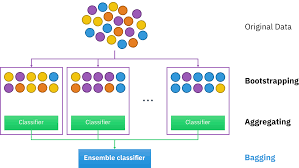
\includegraphics[scale=1]{images/bagging.png}
    \captionsetup{hypcap=false}
    \captionof{figure}{\href{https://en.wikipedia.org/wiki/Random_forest}{en.wikipedia.org}}
    \label{fig:bagging}
\end{center}




Random Forest w przeciwieństwie do SVR nie potrzebuje Feature Scaling. Również MultiOutputRegressor nie jest tutaj potrzebny, ponieważ Random Forest wspiera multioutput. 

\section{Zakończenie}

Jak widac 

\end{document}
